\section{Lexical Models}

In this section we compare different lexical retrieval models
(Section \ref{LexicalModels:Models}) using
offline evaluation (Section \ref{LexicalModels:Evaluation}).

\subsection{Models}
\label{LexicalModels:Models}

%%%%%%%%% It should explain what you have implemented

\subsubsection{TF-IDF}

The tf\textendash idf score is the product of two statistics, 
term frequency and inverse document frequency.
The term frequency indicates how often a given term occurs in a document,
while the inverse document frequency quantifies the specificity of the term.
That is, a term is more specific if it occurs less frequently in the documents of the corpus.  
%
To calculate the tf-idf score of a document for a given query, 
we sum over the tf-idf scores of the individual words in the query.
We use the following formula to calculate these scores: 

\begin{equation*}
tfidf(t,d) = \log(1 + tf(t,d)) \cdot \log\frac{n}{df(t)}
\end{equation*}

We use $\log(1 + tf(t,d))$ instead of the raw term frequency $tf(t,d)$
to account for the fact that relevance	does not increases proportionally with the term frequency. The document frequency is calculated as $df(t) = \#\{d:tf(t,d) > 0\}$.


\subsubsection{BM25}

The BM25 model is slightly more advanced than the tf\textendash idf model;
in addition to term frequency and inverse document frequency
it also includes a component that controls for the document length.
%
To calculate the BM25 score of a document for a given query, 
we sum over the BM25 scores of the unique words in the query.
We use the following formula to calculate these scores: 

\begin{equation*}
BM25(t,d) = \frac{(k + 1) tf(t,d)}{k(1 - b + b \cdot \frac{l_d}{l_{avg}} ) + tf(t,d)} \cdot \log\frac{n}{df(t)} 
\end{equation*}

The values $l_d$ and $l_{avg}$ represent the document length and the average
document length, respectively.
We use $k = 1.5$ and $b = 0.75$ in our evaluation as commonly used default values.
 
\subsubsection{Language Models}

A statistical language model is a probability distribution over word sequences.
To score a given document-query pair, we calculate the query likelihood
$p(q|d)$, which is proportional to $p(d|q)$, 
assuming a uniform prior for $p(d)$.
We use the unigram approximation to calculate the query probability.
That is, we calculate the probability of the query by
multiplying the probabilities of the individual words of the query
(in our actual implementation we sum over the log values to avoid underflow).

We consider three different language models that are different in the way that
they handle smoothing, i.e. adjusting the maximum likelihood estimate to avoid 
zero probability for unseen words.

\paragraph{Jelinek-Mercer}

The Jelinek-Mercer model calculates the probability of a word by
interpolating the language model based on the document with
a background language model based on the full corpus.
The formula is given below.

\begin{equation*}
p_{\lambda}(w | d) = \lambda \frac{tf(w,d)}{|d|} + (1 - \lambda) \frac{tf(w,C)}{|C|}
\end{equation*}


\paragraph{Dirichlet Prior}

Dirichlet prior smoothing also interpolates the maximum 
likelihood estimate with a background model,
but in this case the factor $\lambda$ depends on the document length;
the longer the document the lower the weight of the background component $(1-\lambda)$.
The formula for the Dirichlet model is given below:

\begin{equation*}
p_{\mu}(w | d) = \frac{tf(w,d)}{|d| + \mu}  + \frac{\mu}{\mu + |d|} \frac{tf(w,C)}{|C|}  
\end{equation*}


\paragraph{Absolute Discounting}

Absolute discounting lowers the probability of seen words by substracting a constant value from their counts.
The formula is given below, with $|d|$ the length of the document and $|d|_u$ the number of unique words:

\begin{equation*}
p_{\delta}(w | d) = \frac{\max(tf(w,d) - \delta, 0)}{|d|} + \frac{\delta |d|_{u}}{|d|} \frac{tf(w,C)}{|C|}  
\end{equation*}


\subsubsection{Positional Language Model}

The positional language model differs from the other
language models by the fact that it takes the proximity
of query term occurrences into account. That is,
it rewards documents with matching query terms
close to each other.
%
A language model for each position in a given document 
is calculated from the words in the document discounted
based on their kernel distance to the position.
The final score for a word is determined by the 
propagated score of the word at the best position.
A detailed explanation of the positional language model can 
be found in \cite{PLM}.

We implemented the positional language model
with the best position strategy and dirichlet prior smoothing.
We considered five different kernel functions:
Gaussian, Triangle, Cosine, Circle and Passage.
The formulas for these functions are in \cite{PLM},
except for the `Passage' kernel which
is given by $I(|i - j| <= \sigma)$.
We implemented these kernels with $\sigma = 50$ fixed.
We determine the final score of a document query pair
as the score of the multiplied probabilities of the words 
at the best position (for computational reasons we actually use 
the log of the sum). 


\paragraph{Implementation}

Given a kernel function $k$ and the indicator function 
$c(w,j)$ of the occurence of a word $w$ at position $i$,
the formula for the positional language model is:

\begin{equation*}
p(w|D,i) = \frac{\sum_{j=1}^N c(w,j)k(i,j)}
{\sum_{w' \in V} \sum_{j=1}^N c(w',j)k(i,j)} 
\end{equation*}

Calculating the $p(q|D,i)$ for each position
in order to determine the $p(q|D,i)$ at the 
best position is computationally expensive.
For this reason, we optimized the implementation.

First, we only consider positions in the (inclusive) interval
between the left most occurrence and the right most
occurrence of a query term in the document.
We can savely assume that the best position is within this interval
since the excluded positions have lower probability
than the left and right most positions,
by nature of the kernel functions.

Secondly, we apply the optimization 
described in \cite{PLM} for calculating
$\sum_{w' \in V} \sum_{j=1}^N c(w',j)k(i,j)$.
That is, we actually calculate 
$\sum_{j=1}^N k(j,i)$ which is shown to be equivalent.

Finally, we cache the values that we calculate for 
$\sum_{j=1}^N k(j,i)$. That is,
we build a cache that returns the
value for $\sum_{j=1}^N k(j,i)$ given
a kernel function $k$, a document length $N$
and a position $i$. The cache
significantly reduced the run time
for our test and evaluation runs.
For example, running the positional
language model on the test set takes
approximately TODO! minutes.


\subsection{Offline Evaluation}
\label{LexicalModels:Evaluation}

We compare the retrieval models that we implemented
using offline evaluation. Below we describe
our experimental setup (Section \ref{ExperimentalSetup}), 
the results that we obtained for our lexical retrieval models 
(Section \ref{ResultsLexicalModels}), 
and we provide an analysis of these results 
(Section \ref{AnalysisLexicalModels}).

\subsubsection{Experimental Setup}
\label{ExperimentalSetup}

%%%%%%%%%%%% Test and Validation Data
We create a testset of query-document pairs from a file
containing queries with labeled documents. The labels tell whether
a document is considered relevant or not for the given query.
The testset consists of XXX queries with an average of 
YYY labeled documents per query. 
The average query length is ZZZ words.
%
For optimizing the hyper parameters of our retrieval models
we build a validation set from a second file with different 
labeled query-document pairs. 
The validation set consists of XXX queries with an average of 
YYY labeled documents per query. 
The average query length for the validation set is ZZZ words.


%%%%%%%%%%%% Evaluation pipeline
We run the retrieval models on the query-document pairs from the
testset to score the relevance of the document for the query.
By ordering the documents based on this `relevance' score
we construct a ranking of documents per query.
We then compare our ranking with the relevance labels using
the TREC Eval utility\footnote{\url{https://github.com/usnistgov/trec_eval}}. TREC Eval is the de facto standard way to compute Information Retrieval measures. TREC Eval computes evaluation scores
for a ranking of documents per query, given
ground-truth information regarding the relevance of the documents
for the given query. 

%%%%%%%%%% Metrics: ndcg
TREC Eval produces many different metrics that can be used 
to estimate the quality of a ranking result.
We choose normalized discounted cumulative gain (nDCG) as
our primary metric of interest for comparison of results.
(n)DCG accumulates the gain of documents from the top of the ranking
to the bottom, with the gain of each result discounted at lower ranks.
We compare nDCG scores at rank 10 (nDCG@10) since we consider the top ten results as most important assuming that they 'fit on a page' for a search engine. nDCG is often used to measure effectiveness of web search engine algorithms.

%%%%%%%%%% Metrics: others
In addition to nDCG@10 we also show results for some other metrics,
namely: Mean Average Precision at rank 1000 (MAP@1000), 
recall at rank 1000 (Recall@1000) and Precision at rank 5 (Precision@5).
We show these metrics to give a more complete picture and because they
may be relevant for other search scenarios.


\subsubsection{Results}
\label{ResultsLexicalModels}

We first optimize the hyper parameters of the 
language models and then generate scores for
all retrieval models discussed in 
Section \ref{LexicalModels:Models}.

\paragraph{Optimizing Hyper Parameters}

We optimize the hyper parameters of the language models
by comparing the average nDCG@10 scores on the validation set 
using different values for the hyper parameters.
The results are shown in Figure \ref{Fig:OptimizingHyperParams}.
Unfortunately, the results do not look generalizable and it is
not clear what the best value should be. 

We decided on the actual value that we use in the rest of the experiment
by comparing three values and picking the value that gave the best result.
%
For Jelinek-Mercer we compare the scores for 0.1 (ndcg 0.450),
0.5 (ndcg 0.468) and 0.9 (ndcg 0.468). Based on these results we pick
the parameter value 0.9. 
%
For Absolute Discounting we compare the scores for 0.1 (ndcg 0.454),
0.5 (ndcg 0.461) and 0.9 (ndcg 0.478). Based on these results we pick
the parameter value 0.9. 
%
For Dirichlet prior we compare the scores for 500 (ndcg 0.484),
1000 (ndcg 0.489) and 1500 (ndcg 0.484). Based on these results we pick
the parameter value 1000. 

Jelinek Mercer:
0.1: 0.450
0.5: 0.468
0.9: 0.468

Dirichlet Prior:
500: 0.484
1000: 0.489
1500: 0.484

Absolute Discounting:
0.1: 0.454
0.5: 0.461
0.9: 0.478

\begin{figure}
\centering
\subcaptionbox{Jelinke-Mercer\label{fig_jm_hyperparams}}{%
  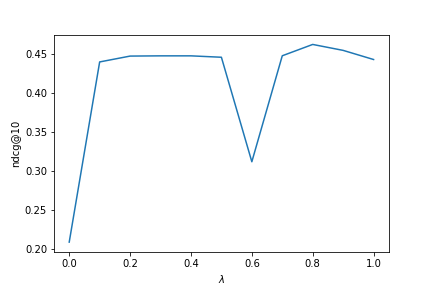
\includegraphics[width=0.25\textwidth]{content/jm_hyperparams.png}%
  }\par\medskip
\subcaptionbox{Absolute Discounting\label{fig_abs_hyperparams}}{%
  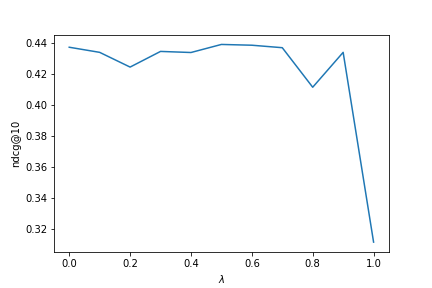
\includegraphics[width=0.25\textwidth]{content/abs_hyperparams.png}%
  }\par\medskip        
\subcaptionbox{Dirichlet Prior\label{fig_dir_hyperparams}}{%
  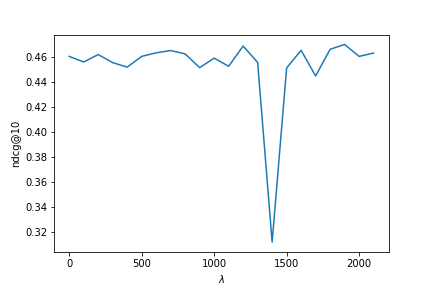
\includegraphics[width=0.25\textwidth]{content/dir_hyperparams.png}%
  }
\caption{Optimizing hyper parameters.}
\label{Fig:OptimizingHyperParams}
\end{figure}


Positional Language Model:

\begin{center}
\begin{table}
\scriptsize
  \begin{tabular}{ r | c | c | c }
                & \thead{Dir. 500} & \thead{Dir. 1000} & \thead{Dir. 1500}  \\ \hline
    \thead{Gaussian} & 0.474 & 0.471 & 0.468  \\ \hline
    \thead{Circle}   & 0.469 & 0.468 & 0.462  \\ \hline
    \thead{Passage}  & \cellcolor{blue!25}0.476 & 0.474 & 0.474  \\ \hline
    \thead{Cosine}   & 0.452 & 0.451 & 0.451  \\ \hline
    \thead{Triangle} & 0.456 & 0.454 & 0.454 \\
    \hline
  \end{tabular}

\vspace{5pt}  
  
  \caption{
     Mean NDCG@10 scores on the validation set for the positional language model,
     using different combinations of kernel functions and dirichlet hyper parameter values. The highlighted cell shows the best combination according to
     this experiment.    
  }
  \label{tbl_plm}
\end{table}
\end{center}


- means
\begin{center}
\begin{table}
\scriptsize
  \begin{tabular}{ r | c | c | c | c | c | c }
                & \thead{TF-IDF} & \thead{BM25} & 
                \thead{JM} & \thead{Dir.} & 
                \thead{Abs. D.} & \thead{PLM} \\ \hline
    \thead{prec@5}      & 0.504 & 0.467 & 0.466 & 0.486 & 0.481 & PLM \\ \hline
    \thead{recall@1000} & 0.983 & 0.983 & 0.983 & 0.983 & 0.983 & PLM \\ \hline
    \thead{map@1000}    & 0.409 & 0.408 & 0.407 & 0.414 & 0.408 & PLM \\ \hline
    \thead{ndcg@10}     & \cellcolor{blue!25}0.490 & 0.479 & 0.465 & 0.486 & 0.473 & PLM \\
    \hline
  \end{tabular}

\vspace{5pt}  
  
  \caption{
     Mean scores on the testset for the following retrieval models:
     TF-IDF,
     BM25,
     Jelinek-Mercer (0.5),
     Dirichlet Prior (1000),
     Absolute Discounting (0.9),
     Positional Language Model (k, mu).
     The highlighted cell shows the maximum score for nDCG@10, our main metric.
  }
  \label{tbl_means}
\end{table}
\end{center}


- pvalues

- manual inspection

\subsubsection{Analysis}
\label{AnalysisLexicalModels}

- Do all methods perform similarly on all queries? Why?

- Is there a single retrieval model that outperforms all other retrieval models (i.e., silver bullet)?